\section{Stoßprozess zweier Kugeln unterschiedlicher Masse}
	
	% Problem/Hypothese, Ansatz 
	Dieser Versuch dient zur Betrachtung der Stoßgesetze. Dazu wird ein ballistischer zentraler Stoß mit Hilfe von zwei aufgehängten Massen untersucht. Es stellt sich die Frage, wie genau die Stoßgesetze mit den gemessenen Werten übereinstimmen. Das Ergebnis dieser Messung zeigt, dass die Theorie mit den ermittelten Werten (nicht) übereinstimmt. % TODO 
	
	\subsection{Methoden}
		
		\subsubsection{Aufbau}
			
		Zum Messen verwenden wir den im Folgenden dargestellten Aufbau. Hierbei handelt es sich um zwei Pendel an denen Kugeln mit unterschiedlicher Masse angehängt sind. Die Schwerpunkte dieser Kugeln liegen auf einer Geraden, sodass ein ballistischer zentraler Stoß durch das Auslenken eines Pendels möglich ist. Abbildung \ref{abb:VersuchsskizzeStoss} stellt dies dar. Dabei ist der Punkt in Ruhelage, wo die beiden Kugeln sich berühren durch $a_0$ gekennzeichnet. Des weiteren sind die Positionen der von $a_0$ gegenüber liegenden Punkte $a_1$ und $a_2$, welche um den Durchmesser der kleineren bzw. größeren Kugel, mit den Massen $m_1$ bzw. $m_2$, von $a_0$ verschieden sind, gekennzeichnet.
		\begin{figure}[ht]
			\centering
			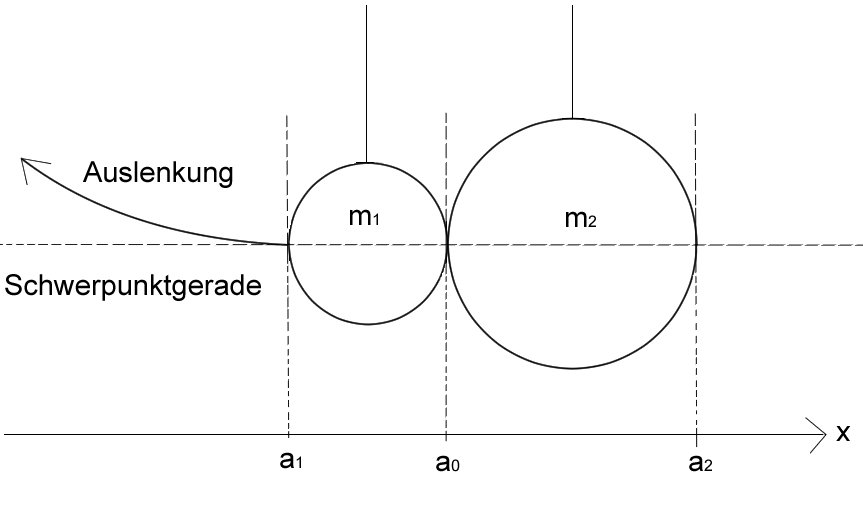
\includegraphics[width=\textwidth]{Kugelstoss.png}
			\caption{Skizzierung des Versuchsaufbaus}
			\label{abb:VersuchsskizzeStoss}	
		\end{figure}
		Dies wurde so gewählt, damit das Messen leichter fällt. Hierzu werden Schiebeblöcke verwendet (vgl. Abb. \ref{abb:VersuchsaufbauStoss}), welche sich auf einem Maß frei bewegen lassen. Damit sind $a_1'$ und $a_2'$ nach dem initialen Stoß leicht zu bestimmen. Die gestrichenen Variablen sollen hierbei die Auslenkung nach dem Stoß beschreiben. Zur Betrachtung im Schwerpunktsystem werden dann die Radien der Kugeln auf die Auslenkungen addiert bzw. subtrahiert (abhängig von der Seite). 
		
		Es werden bei dem Versuch die Auslenkungen $a_1'$ und $a_2'$ für fünf verschiedene Startauslenkungen von $a_1$ und $a_2$ jeweils fünf mal gemessen, wobei die fünf Messwerte für dieselben Auslenkungen gemittelt werden.
		Zudem werden die Pendellänge und Masse der Kugeln bei beiden Pendeln gemessen. Ersteres mit Hilfe eines Maßbands und letzteres über eine Waage.	
		Über die Theorie des ballistischen zentralen Stoßes werden die Massen durch die anderen gemessenen Werte bestimmt und dann mit der gemessenen Masse verglichen. Dazu werden die Auslenkungen gegeneinander aufgetragen und das Verhältnis dabei bestimmt.
				
		\subsubsection{Unsicherheiten}
		
			Zur Berechnung der Unsicherheiten für die gemessenen und ermittelten Werte dient folgende Formel: 
			\begin{equation*}
				u(s) = \pm \sqrt{\sum_{k=0}^{N}\left( \frac{\partial f}{\partial x_i}u(x_i)\right) ^2}. \label{eq:kombUnsicherheit}
			\end{equation*}
			Für die von dem Maß(band) abgelesenen Werte werden Unsicherheiten über eine Dreiecksverteilung und für die von der Waage gemessenen Werte eine Rechteckverteilung verwendet. 
	
	\subsection{Messung}
		
		\begin{table}[ht]
			\caption{Messwerte}
			\centering
			\label{tab:Messwerte}
			\begin{tabular}{c|c}
				{$a_1$} & {}	\\
				\hline
				{}		& {}	\\
				
			\end{tabular}
		\end{table}
	\subsection{Diskussion}
	
	\subsection{Schlussfolgerung}